\documentclass[10pt,journal,compsoc,draftclsnofoot]{IEEEtran}

\usepackage{float}
\usepackage{hyperref}
\usepackage{array}
\usepackage{tocloft}
\usepackage{lscape}
\usepackage{textcomp}
\usepackage{pgfgantt}
\usepackage{geometry}
\geometry{margin=0.75in}

\setcounter{tocdepth}{4}
\setcounter{secnumdepth}{4}

\begin{filecontents}{techreview.bib}
@misc{debugging,
author = {Microsoft},
title = {Standard Debugging Techniques},
url = {https://msdn.microsoft.com/en-us/library/windows/hardware/hh439390(v=vs.85).aspx}
}

@misc{maintainability,
author = {Markus Pizka, Florian Deißenböck},
title = {How to effectively define and measure maintainability},
url = {http://www.itestra.de/fileadmin/Redaktion/Documents/07\_itestra\_define\_and\_measure\_maintainability.pdf}
}

@misc{version,
author = {git},
title = {Getting Started - About Version Control},
url = {https://git-scm.com/book/en/v2/Getting-Started-About-Version-Control}
}

@misc{refactoring,
author = {c2},
title = {What Is Refactoring},
url = {http://wiki.c2.com/?WhatIsRefactoring}
}

@misc{lightmapping,
author = {Alan Baylis},
title = {Lightmapping Tutorial},
url = {http://www.alsprogrammingresource.com/lightmapping\_tutorial.html}
}

@misc{volume,
author = {Josh Beam},
title = {Tutorial - Stenciled Shadow Voumes in OpenGL},
url = {http://joshbeam.com/articles/stenciled\_shadow\_volumes\_in\_opengl/}
}

@misc{shadowMapping,
author = {opengl-tutorial},
title = {Tutorial 16 : Shadow mapping},
url = {http://www.opengl-tutorial.org/intermediate-tutorials/tutorial-16-shadow-mapping/}
}

@misc{gooch,
 author = {ECG Wiki},
 title = {Gooch Shading},
 url      = {https://lva.cg.tuwien.ac.at/ecg/wiki/doku.php?id=students:gooch}
}

@article{gooch2,
 author = {Amy Gooch, Bruce Gooch},
 title = {A Non-Photorealistic Lighting Model For Automatic Technical Illustration},
 url      = {http://artis.imag.fr/~Cyril.Soler/DEA/NonPhotoRealisticRendering/Papers/p447-gooch.pdf}
}

@article{celshading,
 author = {Raul Reyes Luque},
 title = {The Cel Shading Technique},
 url      = {https://raulreyesfinalproject.files.wordpress.com/2012/12/dissertation\_cell-shading-raul\_reyes\_luque.pdf}
}

@article{nonphotshading,
 author = {Marc ten Bosch},
 title = {Non-photorealistic Shading},
 url      = {http://marctenbosch.com/npr\_shading/}
}

@article{hatch,
 author = {Igor Dykhta},
 title = {Hatching and Gooch shading in GLSL},
 url      = {http://www.sunandblackcat.com/tipFullView.php?l=eng\&topicid=27}
}

@article{silhouette,
 author = {OpenGL.org},
 title = {Silhouette Edges},
 url      = {https://www.opengl.org/archives/resources/code/samples/advanced/advanced97/notes/node204.html}
}

@article{nonphotorealisticsilhouette,
 author = {Igor Dykhta},
 title = {Non-photorealistic Rendering (Cel shading)},
 url      = {http://sunandblackcat.com/tipFullView.php?l=eng\&topicid=15}
}

@article{edgedetector,
 author = {DanielRakos},
 title = {Frei-Chen edge detector},
 url      = {http://rastergrid.com/blog/2011/01/frei-chen-edge-detector/}
}

@article{toonshading,
 author = {Sergiu Craitoiu},
 title = {Toon Shading Effect And Simple Contour Detection},
 url      = {http://rastergrid.com/blog/2011/01/frei-chen-edge-detector/}
}

@article{siledges,
 author = {OpenGL.org},
 title = {Silhouette Edges},
 url      = {https://www.usability.gov/how-to-and-tools/methods/user-research/index.html}
}

@misc{codexl,
 author = {gpuopen.com},
 title = {CodeXL},
 url      = {http://gpuopen.com/compute-product/codexl/}
}

@misc{glsl,
 author = {GLSLDebugger},
 title = {GLSLDebugger},
 url      = {http://glsl-debugger.github.io/}
}

@misc{userResearch,
 author = {usability.gov},
 title = {User Research Methods},
 url      = {https://www.usability.gov/how-to-and-tools/methods/user-research/index.html}
}

@article{usabilitynet,
 author = {John Brooke},
 title = {SUS - A quick and dirty usability scale},
 url      = {http://www.usabilitynet.org/trump/documents/Suschapt.doc}
}

@misc{google,
 author = {Google},
 title = {Google Terms of Service},
 url      = {https://www.google.com/policies/terms/}
}

@misc{surveymonkey,
 author = {SurveyMonkey},
 title = {SurveyMonkey and IRB Guidelines},
 url      = {http://help.surveymonkey.com/articles/en\_US/kb/How-does-SurveyMonkey-adhere-to-IRB-guidelines}
}
\end{filecontents}

\begin{document}
\onecolumn

\begin{titlepage}
\null
\vspace{20mm}

\begin{flushleft}
\begin{bfseries}
	\vskip2mm
	\Huge{Technology Review for\\ Better Graphics For A Robotics Grasping GUI}\\
	\vspace{30mm}
	\textbf{\huge Shady Robots} \\
	\vskip2mm
	\large{Group 12}
	\vskip5mm
	\Large{Justin Bibler \\
	Matthew Huang \\
	Daniel Goh \\}
\end{bfseries}

\vspace{15mm}
\Large{CS461: Senior Software Engineering Project} \\
\Large{Fall 2016} \\

\vspace{10mm}

\today

\vfill

\begin{normalsize}
{\bf Abstract:}
Our client is using a simulation to create visuals that are used for online data collection.
This simulation is using outdated libraries which result in outdated graphics.
We, as the supplier, compare and contrast the different technology and methods that will be used during the phase of the project to ensure the project's success.
\end{normalsize}
\end{flushleft}
\end{titlepage}

\section{Introduction}
\vspace{3mm}
The technology review document is used to determine the best approach of implementation for the project. 
Clause 2 lists the references made to other documents.
Clause 3 lists each team member's role in the project and accomplishment goals.
Clauses 4 to 6 are the technology review that is carried out by each team member.
Clause 4 reviews the technology to be used to carry out runtime analysis. performance benchmarks, and best practices to implement shadows.
Clause 5 reviews the best practices to implement shaders, best practices to implement silhouettes, and technology to be used to ensure maintainability of the project's source code.
Clause 6 review usability inspection methods, run user interviews, and tools to analyze the respondents data.

\newpage

\section{Roles}

\subsection{Justin Bibler}
My roles within this project vary from each other, and are not one cohesive singular responsibility.
I have two responsibilities that have a conclusive end, and a responsibility that is maintained throughout the entire project.
The first of the two conclusive responsibilities that I have is to locate where in the code the rendering is happening.
This responsibility is critically important to the entirety of the group, as without knowledge of the location of the rendering function it is difficult to implement shaders.
Secondly, I will be overseeing the implementation of the shadows.
Shadows help define where 3d objects are within a computer simulation, thus our client requested them to be implemented to improve the current graphics.
Finally, my last responsibility is to assure code maintainability.
This means that once our group has finished with the project our additions to the code will be well documented, commented, and easily understandable.
Making it easy for our shader implementations to be changed and adjusted easily to fit our client's needs. \par
Within the "Identification of Rendering loop, Methods of code maintainability, and Shadows" section I compare and contrast three different methods and tools available to conduct and maintain my responsibilities.
How the comparison of methods and tools will be conducted is: I will first explain what the responsibility is and it's relevance to the group and the project.
I will then list a tool or method and how it is used or conducted.
Next, I will list and analyze the benefits and negatives of a tools usage.
At the end of each section I discuss my opinion on the usage of the method.
Finally, after listing all of the available different method and tools I will give my verdict on what will be used.

\subsection{Matthew Huang}
In this team, I'm responsible for the non photorealistic shaders, the silhouettes, and the runtime performance of the modified simulation.
For the shaders, I must make sure that they improve the geometric shape of each object in the simulation.
For the silhouettes, I must make sure that they clearly show where an object's borders are so that user can differentiate shapes from each other.
For the runtime performance, I must make sure that our implementation does not negatively affect the frames per second that the current simulation is running at.
To ensure this, I have researched various debuggers that will help us see what our program is doing during runtime.


\subsection{Daniel Goh}
My role within Shady Robots is to measure the improvement that is implemented into the simulation.
I will also be running the selected inspection method to determine if the project has reached the end goal.
After running the usability inspection, I will be compiling, visualizing and analyze the data set.

Usability inspection methods will be a standard of metrics to determine if the project has reached the end goal.
The goal within this document is to compare and contrast the different available usability inspection methods, data collection tools, and analytical and visualization tools.
After reviewing the various tools, a final verdict of the review is presented at the end of each section.

\newpage

\section{Identification of Rendering loop, Methods of code maintainability, and Shadows}
\large{By Justin Bibler}

\normalsize
\subsection{Identification of Rendering loop}
Our project requires our group to make new implementations into the existing OpenRave code.
However, the location of the rendering functions within OpenRave are not entirely know to our client.
Therefore, the responsibility of locating these functions has been given to our group.
This responsibility is very important to the entirety of the project.
Most of our new implementations into the code will be reliant on the use of shaders;
 if the location of the rendering functions are unknown to us it would be extremely difficult for us to make good shader implementations.
Thus, to identify the location of the rendering functions the three most fitting methods would be: Reading Static Code, debugging, external references, and documentation.

\subsubsection{Reading Static Code}
This is a very basic method in which a programmer simply reads over and reviews static code.
In this case the OpenRave source code would be read over to identify how the rendering function is working.

Benefits of Reading Static Code:
\begin{itemize}
\item The entire system can be understood at a very low level.
\item Locations of specific functions within the code can be identified.
\item Exact implementation of functions can be understood.
\end{itemize}

Negatives of Reading Static Code:
\begin{itemize}
\item This method can become very time consuming depending on the size and complexity of the code.
\item Code may difficult to read depending on how it is implemented.
\item Inefficient, a programmer will most likely have to flip around multiple source files to figure out how things are working together.
\end{itemize}

\paragraph{Discussion}
%\vspace{3mm}
Reading static code might be too simple of a method to conduct by itself.
It would definitely help me get a good understanding of how the code is function.
However, as mentioned in the negatives of this method it may be too time consuming.
The source code for OpenRave is quite large, and I have minimal experience working on a project this large scale so it would be difficult for me to jump right in and simply read code.
Perhaps if this method were to be paired with another it could be useful.

\subsubsection{Debugging}
Debugging is a process where a programmer will use tools, and programming methods to locate errors in code.
Many different forms and tools exist to conduct debugging.\cite{debugging}
Thus, I will narrow the scope down to one specific form a debugging: breakpoints, and step through.
Breakpoints stop an executable and breaks into the debugger.
This allows a programmer to analyze the code and execute debugger commands.\cite{debugging}

Benefits of Debugging:
\begin{itemize}
\item Lots of available tools.
\item Lots of available methods.
\item Powerful control over code.
\item Executable within most modern IDEs.
\end{itemize}

Negatives of Debugging
\begin{itemize}
\item Difficult to conduct on large projects.
\item Stepping through code can become time consuming.
\end{itemize}

\paragraph{Discussion}
%\vspace{3mm}
Debugging is a good method that would help me accomplish my goal.
If I were to use a method such as breakpoints and step through code at certain points, it could become a very helpful resource to use.
However, due to the size of the program I am not exactly sure how easy it will be to debug.

\subsubsection{External References, and Documentation}
Much like reading static code this is a very simple and obvious method that can be used to locate the rendering function.
This method is where a programmer will read through the available documentation to understand how the system works.
In this method a programmer will also contact other programmers who are working on the code currently, or have worked on the code in the past.
With the intention of receiving guidance on how the system works.

Benefits of External References, and Documentation:
\begin{itemize}
\item Easy to get answers to specific questions.
\item Documentation gives a good understanding of the entirety of a system.
\end{itemize}

Negatives of External References, and Documentation:
\begin{itemize}
\item There may be no documentation.
\item External sources may not exist.
\item Past programmers may be unresponsive.
\end{itemize}

\paragraph{Discussion}
%\vspace{3mm}
It's quite obvious that this is one of the best methods.
Because I am attempting to find a specific function within the code, referring to the documentation and external sources is a good choice.
Along with this, the GitHub that is being used for OpenRave has a couple of active users so it would be relatively easy to contact another programmer who is more knowledgeable to assist me.

\subsubsection{Verdict}
My verdict on methods for identifying the rendering function is that all of the proposed methods are useful.
I will most likely begin my search in the documentation then use the knowledge I gained from the documents to traverse through the source code.
This is because as helpful as the documentation will be, it's required of me to read the actual code so I will have an even better understanding of it.
If I am unable to locate the rendering function through documentation and by reading the code.
I will reach out to other programmers within the GitHub group for assistance.
As a last result, I will be using debugging techniques to traverse through the code in attempts to locate the function.

\newpage
\subsection{Methods of code maintainability}
The goal of creating maintainable code is to increase cost effectiveness.
This means that whenever a new change needs to be made to the system, due to how the code is a designed and constructed this change will take a minimal amount of time.\cite{maintainability}
Maintainability is important to our code, because our client wishes to have the ability to easily change and adjust our implementation of shaders into the system.
Thus our implementations into the code should use methods that allow for an increase in the ability to quickly understand and modify code.
These proposed methods are: Version Control, Refactoring, Documentation, and Commenting.

\subsubsection{Version Control}
Version control has become increasingly easy to maintain with the popularity of version control tools such as GitHub.
Using version control allows for users to make copies of repositories to either use for personnel use or make altercations.
This practices gives protection to the code, such as if programmer losses or makes a devastating alteration to the code.
That programmer doesn't have to worry much, because they know they can pull unmodified working code from the repository.\cite{version}

Benefits of using Version Control:
\begin{itemize}
\item Source code is easily accessible.
\item General tests can be defined to update stable versions of code in a repository.
\item Code is safe to accidental deletion, or introductions of major bugs.
\end{itemize}

Negatives of using Version Control:
\begin{itemize}
\item There aren't really any negatives
\end{itemize}

\paragraph{Discussion}
\vspace{3mm}
Using version control is a obvious powerful tool.
It essentially protects code from being lost or broken.
If a programmer accidentally introduces a large bug into the system, then with version control it is very easy to step back and pull older versions of the code.
In the case that a programmer accidentally deletes their code, it's easy for them to go back and simply pull it from the repository again.
Using version control most assuredly would help increase code maintainability.

\subsubsection{Refactoring}
Refactoring is a process in which code is altered in a manner such that it does not change how the external behavior of the system works.\cite{refactoring}
In the case of this project, refactoring would be used after our group has created a working implementation of our clients request.
We would go back into our code, and adjust our code so that it might be smaller, more readable, and in most cases reusable.
Such as refactoring repeated code into a singular function that can be used in multiple locations of the code.

Benefits of using Refactoring:
\begin{itemize}
\item Easy to do.
\item Cuts down code size.
\item Reusable functions can be implemented and used in different locations of code.
\item Maximizes runtime.
\end{itemize}

Negatives of using Refactoring:
\begin{itemize}
\item After a lot of refactoring code can become less readable.
\end{itemize}

\paragraph{Discussion}
%\vspace{3mm}
Refactoring is a good method to maximize code, especially when refactoring repeated code into new functions.
If I were to refactor our implementations into the code with the client's desires in mind.
I could most likely make it simple for them to adjust, and reuse functions throughout the program if they desire to change it.

\subsubsection{Documentation, and Commenting}
Documentation and Commenting allows new programmers to quickly get a grasp on the code.
In the case of comments, a programmer is able to quickly understand intentions behind functions and certain operations within the code to get a better understanding of how the system works.
And documentation of the code allows a programmer to have references to many questions related to the code.

Benefits of Documentation, and Commenting:
\begin{itemize}
\item New programmers have references to the what, where, and why of code.
\item Good commenting allows a programmer to get a better understanding of the code while directly reading the code.
\item Programmers have references of how to use functions, either in the comments of a function or in the documentation.
\end{itemize}

Negatives of Documentation, and Commenting:
\begin{itemize}
\item Too much, and useless comments can make code look clustered and sloppy.
\item Writing documents can become time consuming depending on the size of system.
\end{itemize}

\paragraph{Discussion}
%\vspace{3mm}
Early in the document I talked about how I would be using documentation to help find the rendering functions within the OpenRave code.
Thus, I personally find using documentation very helpful.
I personally would prefer to focus more heavily on documenting our additions outside of the code rather then simply using comments.
This is because documents are simply and easier reference.

\subsubsection{Verdict}
Each of these methods has it's usefulness that I will utilize to keep the system maintainable.
Version control allows our group to make alterations to the code without fear of losing stable versions.
This also allows for our client to come in and make their own alterations later in the future after the project is finished.
In regards to documentation, and commenting.
I will be recording all the changes and additions we make to the source code.
This allows our group, and our client to have easy references to usable functions within the system.
Finally, I will be using refactoring when I see it fit to be used.
Our group is not expecting to make such massive alterations into the existing code that refactoring would have a major impact.
I also do not intend to refactor the currently written OpenRave code.

\newpage
\subsection{Shadows}
Shadows are used to help understand where in an object is within a 3d simulation.
However, the current graphics used in OpenRave do not contain shadows.
So our client has requested that we implement shadows into the current system.
My proposed methods are: Light mapping, Shadow volumes, and Shadow mapping.

\subsubsection{Light mapping}
A light map is simply a texture that contains information about the lighting. 
In most cases a light map is rendered before the program is executed to speed up the programs runtime.
Essentially, this light map is blended with textures that are intended to be lit to give off an illusion of lighting, and shadows.\cite{lightmapping}

Benefits of using Light mapping:
\begin{itemize}
\item Easy to implement.
\item Can be pre-rendered to increase runtime
\end{itemize}

Negatives of using Light mapping:
\begin{itemize}
\item Lighting is not dynamic.
\end{itemize}

\paragraph{Discussion}
Light mapping seems like a good choice for doing lighting and shading for static objects in OpenRave.
However, because the simulation contains moving 3d objects it will most likely need more dynamic shadows.

\subsubsection{Shadow Volumes}
This form of shadowing takes advantage of the stencil buffer in OpenGL.
Essentially, a shadow volume is a volume in space that contains every point in which an object could be shaded.
Objects that collide with the shadow volume should generate shadowing on their surface according to the shadow volume.
This is done by rendering objects shadowed pixels with different stencil values compared to their non-shadow pixels. \cite{volume}

Benefits of Shadow Volumes:
\begin{itemize}
\item Dynamic.
\item Relatively lightweight.
\end{itemize}

Negatives of Shadow Volumes:
\begin{itemize}
\item Doesn't generate the best looking shadows.
\end{itemize}

\paragraph{Discussion}
\vspace{3mm}
This for of creating shadows seems relatively simple for my skill level.
Along with this it's dynamic, and lightweight which are both good qualities our group is looking for in our shadow implementations.

\subsubsection{Shadow maps}
Shadow mapping is kind of like light mapping.
Shadow mapping works by rendering a scene twice.
In the first render, only the depth of each fragment is computed.
In the second render, the scene is rendered normally.
However, the information computed in the first render is used to calculate whether or not an object has fragments in front of it relative to the light source.
If a fragment has a fragment from the first render blocking it, a shadow should be placed displayed. \cite{shadowMapping}

Benefits of Shadow Mapping:
\begin{itemize}
\item Shadows are dynamic.
\item Shadows will look good because they are fragment based.
\end{itemize}

Negatives of Shadow Mapping:
\begin{itemize}
\item Requires scene to be rendered multiple times.
\item Worse runtime.
\end{itemize}

\paragraph{Discussion}
\vspace{3mm}
Shadow mapping seems great, it also seems like it would create the best looking shadows for the simulation.
However, shadow mapping would most likely greatly increase the runtime of the program and be detrimental to the FPS.

\subsubsection{Verdict}
I think that the shadow volume implementation would be the best to implement into the system.
This is because it offer acceptable looking dynamic shadows, without sacrificing too much runtime and FPS.
It would be great if we could implement the shadow mapping, but the computers that the simulation will be frequently ran on does not have the best GPU.
Making shadow mapping a bad choice.

\newpage

\section{Non photorealistic shading, silhouettes, and optimization - run time analysis}
\large{By Matthew Huang}
\normalsize
\subsection{Non photorealistic shading}

\subsubsection{Gooch Shading (Cool to Warm Shading)}
Gooch shading, developed by Amy Gooch, Bruce Gooch, Peter Shirley, and Elaine Cohen, is a non photorealistic shading model for rendering objects in a technical illustration style. \cite{gooch}
In Gooch Shading, the following characteristics are prominent:
\begin{itemize}
\item Edge lines are drawn with black curves.
\item 3D objects are shaded using color intensities that are far from black or white. Instead, the warmth or coolness of a color indicates its relationship to the surface normal.
\item A single light source provides white light for the object.
\item Shadowing is not shown.
\item Metal objects are shaded as if very anisotropic
\end{itemize}
The colors used in Gooch shading have distinct tones and temperatures.
The color tones are created by adding either gray to the color or by adding the color's complement to the color. The temperature of the color is defined to be warm (red, orange, yellow), cool (blue, violet, green), or temperate (red-violet, yellow-green). Shading with these colors will allow for tone scaled object color along with a warm-to-cool undertone. An example of a Gooch Shaded Object is provided in Figure 1 below. \cite{gooch2}

\begin{figure} [H]
  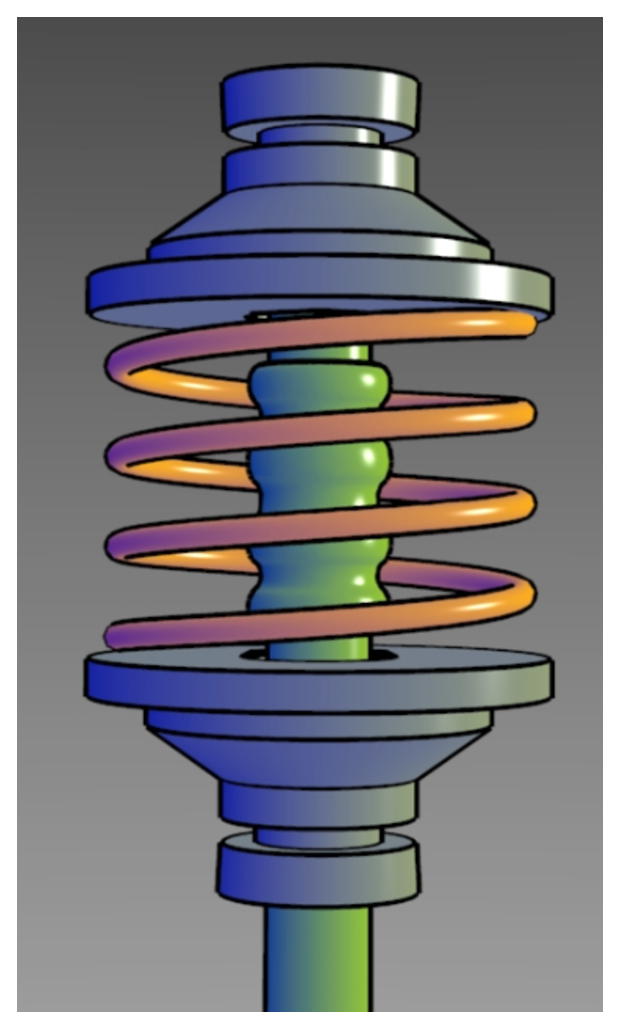
\includegraphics[scale=0.5]{one.eps}
  \caption
{ \newline \hspace{\linewidth}
Gooch shaded model showing the implementation of black edge lines combined with curve highlights and warm to cool hue shifts.}
  \label{fig:one}
\end{figure}

\subsubsection{Cel Shading}
A common type of non photorealistic shading that is primarily used to give 3D objects in computer graphics a flat, 2D look. 
It accomplishes this by using fewer shading colors as opposed to the traditional shading gradient
Additionally, in cel shading, color hues are distinct and do not blend. \cite{celshading}
This is implemented by defining constant light intensities at certain regions and is responsible for the main visual difference between realistic shading and cel shading. 
The lighting in cel shading is done per pixel and can be implemented in either the vertex or fragment shader. \cite{nonphotshading} 
Figure 2 below illustrates the differences between cel and realistic shading.

\begin{figure} [H]
  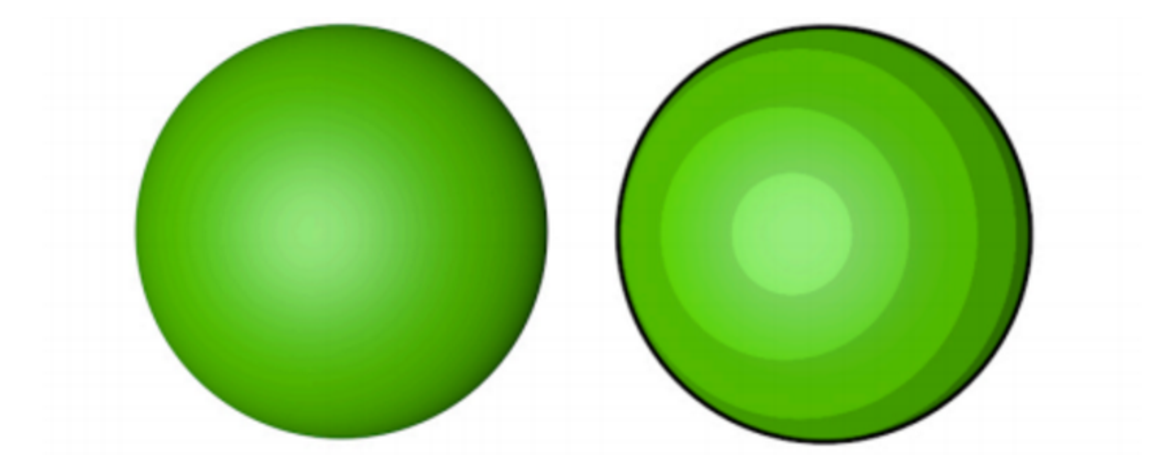
\includegraphics[scale=0.5]{two.eps}
  \caption
{ \newline \hspace{\linewidth}
On the left is an object shaded using realistic shading. 
Observe that there is a wide range of shading colors and that colors blend together. 
On the right is an object shaded using cel shading.
Notice that color hues are few in number and are distinct from each other (I.E. do not blend).}
  \label{fig:two}
\end{figure}

\subsubsection{Hatching}
A non photorealistic shading technique that does shading by drawing multiple hatches (parallel lines) to highlight darker parts of an object. 
The general rule of thumb is the darker the area, the more hatches are drawn there. 
The length, width, and distance between hatches are defined by the developer.
If the hatches are not parallel and instead cross, then it is called cross-hatching. \cite{hatch}
Drawing hatches with different angles can help with emphasizing curves in an object.
To implement hatching, textures of different levels of hatching are first created. 
After that, these texture can then be sent to the fragment shader and be assigned based on the lighting of the object.
Figure 3 what a 3D cat would look like if it was shaded using hatching.

\begin{figure} [H]
  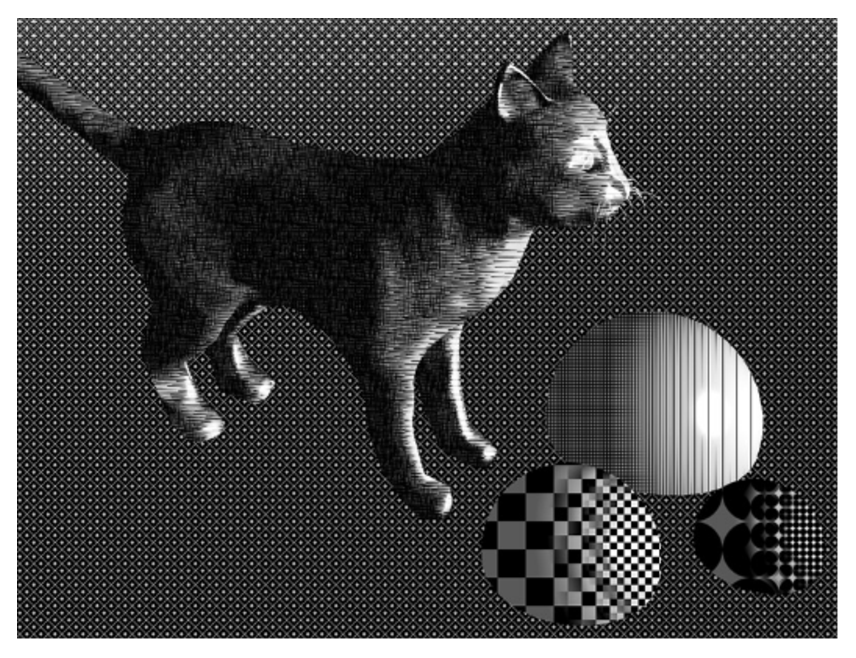
\includegraphics[scale=0.5]{three.eps}
  \caption
{ \newline \hspace{\linewidth}
3D cat drawn using simple hatching. Notice that the number of hatches drawn is used to highlight the curves of the cat and is based on the light position.}
  \label{fig:three}
\end{figure}

\subsubsection{Goals}
Our client wants the shading to primarily highlight object shape. 
This entails focus on emphasizing the curves of objects, 
They also want all parts of any 3D rendered object to be visible if it is within view.
This would mean that no piece of an object should be completely black as this would possible confuse the object's shape.

\subsubsection{Criteria}
These technologies will be primarily judged based on how well they highlight object shape and visibility. 
Additionally, how well each are documented will be considered.
Speed, resource cost, and implementation flexibility will also be factored in but at a lower priority. 
This is because the speed and cost of shading implementations are more dependent on the specific implementation rather than the type of shading.

\subsubsection{Table}
\begin{center}
\begin{table}[H]
\begin{tabular}{ | m{7em} | m{7em} | m{7em} | m{7em} | m{7em} | m{7em} |  } 
\hline
\textbf{Technology}  & \textbf{Highlight Shape} & \textbf{Object Visibility} & \textbf{Documentation} & \textbf{Speed \& Cost} & \textbf{Flexibility} \\ \hline
Gooch Shading & Shape highlighted using warm to cool colors tones. & No parts of the 3D object is completely blacked out. & Well documented. Original paper detailing Gooch Shading available online. & Uses equations to calculate tones of a color. Will mostly depend on specific implementation. & Can be implemented with fragment or vertex shader.  \\ \hline
Cel Shading & Shape highlighted using few shading colors. Color hues do not blend which creates a 2D look for the shape. & Object areas have constant light intensities so they aren't typically completely black. & Widely used and well documented. Many pieces of sample code exist online. & Fast and efficient due to fewer shading colors and constant light intensities. & Lighting can be done using vertex or fragment shader.  \\ \hline
Hatching & Shape highlighted by using textures with different number of hatches. The darker the area, the more hatches. & Darker areas of an object have more hatches drawn there meaning parts of it could be completely black. & Not as common as cel or Gooch shading but documentation still exists. & Depends on implementation. Hatches typically drawn using textures and lighting equations. & Must use both vertex and fragment shader. \\ \hline
\end{tabular}
\newline
\caption{Comparing non photorealistic shading technologies}
\label{table:nonphoto}
\end{table}
\end{center}

\newpage

\subsubsection{Discussion}
All three shaders do well at highlighting object shape. 
For our purposes, however, Gooch shading and Hatching do a better job since they allow for the object to retain its 3D shape. 
Cel shading makes objects look 2D which, for us, is bad.
Gooch and cel shading both do well at keeping full object visibility. 
Hatching has the possibility of completely blackening certain parts of objects which means visibility may be a problem.
Cel shading is the most well documented since it is the most common type among the 3. 
Gooch is not far behind with its documentation widely available online.
Hatching is the least well documented, but resources still exist online.
Cel is likely the fastest and most efficient among the 3 shaders but the others aren't far behind.
Gooch and cel shading can be implemented using either the vertex or fragment shader while Hatching must use both.
This is not much of a problem, however, since our implementation will likely use both anyways.

\subsubsection{Choice}
For our purposes, Gooch shading is the best option. 
It does a great job at highlighting object shape while also guaranteeing full object visibility. 
Additionally, good documentation exists online for it so getting started won't be an issue.
The other two types of shading weren't selected because they didn't highlight both object shape and visibility.
Cel doesn't do well at highlighting 3D curves and Hatching does a poor job at showing object visibility.

\newpage

\subsection{Silhouettes}

\subsubsection{Stencil Buffer Technique}
Technique for rendering a silhouette edge around a 3D object using the stencil buffer.
This technique can draw the silhouette of an object before or after the object is drawn.
In this algorithm, the object is drawn 4 times; each time displaced by 1 pixel in the x or y direction. \cite{silhouette}
This offset is done in windows coordinates and can be implemented by changing the viewport coordinates each time.
The algorithm, in detail, is provided below [6]:
\begin{enumerate}
\item If you want to see the object itself, render it in the usual way.
\item Clear the stencil buffer to zero.
\item Disable writing to the color and depth buffers
\item Set the stencil function to always pass, set the stencil operation to increment
\item Translate the object by +1 pixel in y, using glViewport()
\item Render the object
\item Translate the object by -2 pixels in y, using glViewport()
\item Render the object
\item Translate by +1 pixel x and +1 pixel in y
\item Render
\item Translate by -2 pixel in x
\item Render
\item Translate by +1 pixel in x. You should be back to the original position.
\item Turn on the color and depth buffer
\item Set the stencil function to pass if the stencil value is 2 or 3. Since the possible values range from 0 to 4, the stencil function can pass if stencil bit 1 is set (counting from 0).
\item Rendering any primitive that covers the object will draw only the pixels of the silhouette. For a solid color silhouette, render a polygon of the color desired over the object [6].
\end{enumerate}

\newpage

\subsubsection{Silhouettes using Polygonal offsets}
A common technique to draw silhouettes often used in cel shading (note cel shading itself not necessary to use this technique).
To implement these silhouettes, first render an enlarged version of the object with a constant color (black). \cite{nonphotorealisticsilhouette}
After that, render the object again but with its normal size and a different color over the top of the enlarged version.
This process is shown visually in Figure 4 below:

\begin{figure} [H]
  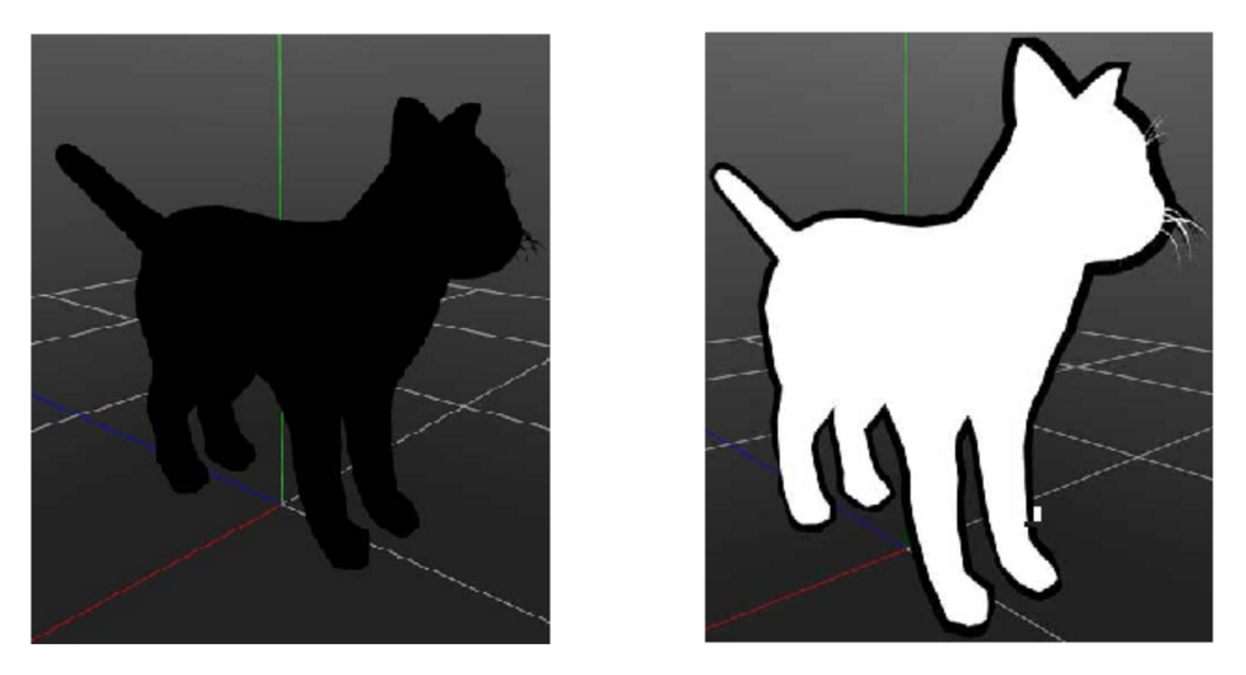
\includegraphics[scale=0.5]{four.eps}
  \caption
{ \newline \hspace{\linewidth}
On the left is the scene after the first rendering. The scene displays an enlarged version of the object drawn only in black. On the right is the scene after the second rendering. The second rendering draws the object (in white) with its normal size over the enlarged version creating the silhouette.}
  \label{fig:four}
\end{figure}

\subsubsection{Edge Detection Silhouettes}
The basic idea of this technique is find all the front facing edges of the object and to place them in a list.
There are multiple algorithms out there to do this such as the Frei-Chen edge detection algorithm. \cite{edgedetector}
After the edge list is created, draw along the list in black (or any other desired color) and the silhouette will be drawn. \cite{toonshading}
The main part of this technique is the edge detection. 
Although multiple algorithms exist, some are exceedingly slow and others are difficult to implement.

\subsubsection{Goals}
Silhouettes should define an object's borders. 
In other words, they define where an object begins and ends.
Their primary purpose is to help differentiate objects in the scene from each other.
This will assist in defining an object's position within the scene.

\subsubsection{Criteria}
These silhouettes will be judged on smoothness, ease of implementation, efficiency, flexibility, and how well documented it is.
Smoothness is self explanatory; silhouettes should not appear jagged when zoomed in on.
Ease of implementation varies greatly between different silhouette techniques; implementation time should only be increased if the benefit is significant.
Efficiency will be determined by how the silhouette is created. Some techniques create it by drawing the object twice, others create it by traversing the object's vertices.
Flexibility is measured by how the silhouette behaves under different situations. For example, does it work when objects overlap?

\subsubsection{Table}
\begin{center}
\begin{table}[H]
\begin{tabular}{ | m{7em} | m{7em} | m{7em} | m{7em} | m{7em} | m{7em} |  } 
\hline
\textbf{Technology}  & \textbf{Smoothness} & \textbf{Implementation Difficulty} & \textbf{Efficiency} & \textbf{Flexibility} & \textbf{Documentation} \\ \hline
Stencil Buffer Technique & Based on how the original object was drawn since its vertices to create the silhouette. & Involves messing with the Stencil Buffer. Algorithm to implement these silhouettes provided online. & Draws the object 4 times. & Handles overlapping objects well. It can display just silhouette edges or edges and borders. & Well documented on OpenGL websites and other sources.  \\ \hline
Polygonal offset & Based on how the original object was drawn since its vertices to create the silhouette. & Easy. Simply draw the object twice but with an offset on one of them. & Draws the at least twice. & Struggles when objects overlap since the silhouette is a background object. & Well document since it is easy to implement and commonly used in cel shading.  \\ \hline
Edge Detection & Based on how the original object was drawn since its vertices to create the silhouette. & Varies depending on the edge detection algorithm used. & Traverse through every vertex of the object. Efficiency also dependent on edge detection algorithm. & Handles overlapping objects well since separate objects have their own edge lists. & Not well documented. Resources mostly come from forum posts and stackoverflow questions. \\ \hline
\end{tabular}
\newline
\caption{Comparing silhouettes technologies}
\label{table:silhouettes}
\end{table}
\end{center}

\newpage

\subsubsection{Discussion}
All three silhouette drawing methods have the ability to create smooth silhouettes since they are all based on how the object was drawn.
The polygonal offset method is by far the easiest to implement since it is just drawing the object twice but with an offset.
The stencil buffer technique has a detailed and clear algorithm for its implementation so it's simple to implement too.
The edge detection method is less clear due to lack of solid documentation.
The polygonal offset and edge detection methods are similar in efficiency while the stencil buffer technique is the most inefficient (since it has to draw the object four times).
The only method that struggles with overlapping objects is the polygonal offset method. 
This is significant since overlapping objects are common in 3D scenes.
All three methods have resources online, but the edge detection method is the least well documented.

\subsubsection{Choice}
The stencil buffer technique is the best method for our purposes.
It is well documented so implementing it will be straightforward.
Additionally, it is flexible in what it displays (silhouette edges, borders, etc.) and when it is applied (after object is drawn or before). 
The only draw back is its efficiency since it has to draw the object four times.
There are, however, modifications to the algorithm that can reduce the number of times it has to draw to two. \cite{siledges}
The edge detection case was not chosen because it is not well documented.
The polygonal offset choice, while easy to implement and well documented, was not chosen because it lacked flexibility.

\newpage

\subsection{Optimization - Run time analysis}

\subsubsection{CodeXL}
A powerful OpenGL and OpenGL ES debugger that was once called gDEBugger before it was bought out by AMD.
It traces application activity on the OpenGL API which will assist with finding bugs and boosting performance.
CodeXL can be applied to a variety of applications and works on Windows and Linux platforms.
Using it is as simple as just running the application in the debugger.
Additionally, CodeXL has a multitude of features that will assist in the debugging process such as static shaders analysis, GPU profiling, and power profiling. \cite{codexl}
CodeXL is available on github and is free to use.

\subsubsection{GLSL-Debugger}
An open source fork of the glslDevil project.
GLSL-Debugger is a tool for debugging OpenGL programs.
Key features include tracing OpenGL programs, visual GLSL step-by-step debugging, support for Linux and Windows, and record and playback OpenGL traces [11].
The source code is available online for free but requires the user to compile it.
Instructions for how to do this is shown on their website.

\subsubsection{GLIntercept}
GLIntercept is a OpenGL function call interceptor available for the windows platform. \cite{glsl}
To use it, user must copy certain install files (opengl32.dll and a gliConfig.ini) to the executable folder and then edit the gliConfig.ini file to their liking.
Additionally, GLIntercept has a variety of feature including function call logging, saving and tracking of shaders, saving and tracking of display lists, function stats, and more.
GLIntercept is available on github for free.
Importantly note that this debugger may not work on advanced features in OpenGL 3.0+ due to it being developed using the OpenGL 1.0-2.1 debugger [12].

\subsubsection{Goals}
The goal of this runtime analyzer is to improve application performance by tracing where resources are being used in the program.
In general, our modifications should not slow down the current implementation as that would hurt the smoothness of the simulation.
This analyzer will help track the changes our modifications are making to the program.

\subsubsection{Criteria}
The debuggers will be judged based on relevant features, usability, and documentation.
Relevant features include function call tracing, data structure tracking, available platforms, etc.
Usability is measured by how easy it is to install and use.
Documentation is measured by how many resources on the debugger are available online.
The first two factors will be of higher priority than the third because not having certain features is much more important than amount of documentation.

\subsubsection{Table}
\begin{center}
\begin{table}[H]
\begin{tabular}{ | m{7em} | m{7em} | m{7em} | m{7em} | m{7em} | m{7em} |  } 
\hline
\textbf{Technology}  & \textbf{Program tracing and tracking} & \textbf{Other Relevant Features} & \textbf{Usability} & \textbf{Available Platforms} & \textbf{Documentation} \\ \hline
CodeXL & Included  & Static Shader Analysis. GPU and Power profiling. & Easy to use and download. Quick start guide available for download.
Uses a GUI to display resource consumption. & Windows and Linux. & Well documented with a quick start guide available.  \\ \hline
GLSL\-Debugger & Included & None & Source code available online. Must build and compile yourself. Uses a GUI to display program tracing. & Windows and Linux. & Not very well documented. Their website has enough documentation to get the debugger built.  \\ \hline
GLIntercept & Included & Resource leak tracing, tracking of error states, function timer logs. & Source code available online. Must copy files over and edit certain files to debug. No GUI. & Windows. & Well documented. Github page has detailed list of features and short tutorial on how to use it. \\ \hline
\end{tabular}
\newline
\caption{Comparing run time analysis technologies}
\label{table:runtime}
\end{table}
\end{center}

\newpage

\subsubsection{Discussion}
As far as features go, all of the debugger have the minimum necessary features to warrant use (I.E. program tracing).
CodeXL has the most available features, but they may not all be useful to us.
GLSL-Debugger has the fewest features while GLIntercept is somewhere in the middle.
In the usability department, CodeXL ends up on top.
It's not only easy to install, but it also comes with a useful GUI for debugging.
GLSL-Debugger also comes with a GUI, but it is trickier to get working.
GLIntercept has no GUI which hurts its overall usability.
For available platforms, the only debugger that doesn't work on Linux is GLIntercept.
This is significant as it factors into other parts of our project such as maintenance.
When it comes to documentation, CodeXL once again comes out on top.
Its provided quick start guide shows useful examples on how to install and use the application.
GLIntercept has good documentation, but no examples while GLSL-Debugger only provides screenshot for how to use it.

\subsubsection{Choice}
CodeXL is the best debugger for our purposes.
It provides many useful features for us to use while also being user friendly. 
Additionally, good documentation for it is available online; the aforementioned quick start guide is especially useful.
The GLIntercept debugger was not chosen because it was limited on platform.
The project must work on Linux so having a debugger that doesn't work on Linux would be a hassle.
GLSL-Debugger was not chosen because it was too simple (in terms of features) and not very well documented.

\newpage

\section{Usability inspection methods, how to carry out the selected inspection method, and the tools to analyze the gathered data}
\large{By Daniel Goh}

\normalsize
\subsection{Usability Inspection Methods}
Usability inspection will be carried out to measure the improvement between the starting and the end phase of the project.
Usability.gov lists multiple usability inspection methods that can be used to determine the usability of an interface. \cite{userResearch}
The three main inspection methods that suits this project scope include: Individual Interviews, Online Surveys, and System Usability Scale (SUS).
This section will be used to review various inspection methods and select one that will best suit this project.

\subsubsection{Individual Interviews}
An individual interview is an inspection method in which a interviewer talks to the participant for 30 minutes to an hour.
During this interview, the interviewer is tasked to gain a deeper understanding of the participants.
This includes taking note of the participant's attitudes, beliefs, desires, and experiences.

Guidelines to conduct individual interviews as defined by usability.gov are as follows:
\begin{itemize}
\item Define the aim of the study and select relevant participants.
\item Prepare interview protocol which includes questions and probes to use during the interview.
\item Create a comfortable interview situation by asking questions in a neutral manner and be attentive for probe queues.
\item Get permission to tape interview session, and have one or more note takers during the interview.
\end{itemize}

Benefits of Individual Interviews:
\begin{itemize}
\item Researchers will be able to gain a better understanding of individual participants.
\item Researchers will be able to observe the participant's body language and facial emotions during the interview.
\item Researchers will be able to receive additional insights that might not have occurred to the interviewer.
\end{itemize}

\subsubsection{Online Surveys} 
An online survey is a form of feedback that is done over the internet.
This inspection method is structured as a questionnaire, and is published online to gather feedback from a broad audience.
The data is then stored within a database, and a survey tool is used to analyze the data.

Guidelines to conduct individual interviews as defined by usability.gov are as follows:
\begin{itemize}
\item Identify purpose of the survey.
\item Determine and select target audience that will best suit the project.
\item Identify methods to collect data and limitations to data collection.
\item Create brief surveys.
\item Provide estimated time to completion up front, and show progress of survey to participants.
\item Mix in open-ended questions with closed questions.
\item Allow participants to choose to answer in-depth questions through a follow-up session.
\end{itemize}

Benefits of Online Surveys:
\begin{itemize}
\item Researchers will be able to reach to a broader audience.
\item Researchers will be able to learn who the users are.
\item Users will be more willing to participate as it would not take up too much time.
\item A wide variety of survey tools are available online.
\item Cost efficient for researchers.
\end{itemize}

\subsubsection{The System Usability Scale} 
The System Usability Scale (SUS) is a tool created by John Brooke in 1986.
The SUS method is structured as a ten item questionnaire that requires users to rate individual items with five response options; from Strongly agree to Strongly disagree.

Guidelines to conduct System Usability Scale as defined by usability.gov and UsabilityNet.org are as follows:
\begin{itemize}
\item Participants should not spend time thinking about items for a long time, instead they should record their immediate response. \cite{usabilitynet}
\item The questionnaire are defined and covers the need for support, training, and complexity of system usability.
\item Data gathered through this method needs to be "normalized" to produce a percentile ranking.
\end{itemize}

Benefits of The System Usability Scale:
\begin{itemize}
\item Easy to scale to administer to participants.
\item Study can yield reliable results, even on small sample sizes
\item The System Usability Scale is an industry standard, and is credible in differentiating usable systems from unusable ones.
\end{itemize}

\subsubsection{Goals}
The goals of running usability inspections is used to determine if our team was able to successfully improve the current simulation's visuals.

\subsubsection{Criteria}
The criteria of selecting a suitable usability inspection method is as follows:
\begin{itemize}
\item Needs to easily allow participants to view and choose between two pictures (old visualization and new visualization)
\item Needs to allow the team to get at least 20 respondents within 6 weeks
\item Needs to take less than 10 minutes of the participants time to increase participation willingness
\end{itemize}

\subsubsection{Table}
\begin{center}
\begin{table}[H]
\begin{tabular}{ | m{10em} | m{15em} | m{15em} | m{15em} |  } 
\hline
\textbf{Methods}  & \textbf{Time needed of team to conduct method per session} & \textbf{Time needed of participant to participate} & \textbf{Estimated amount of people that can be reached within 6 weeks} \\ \hline
User Interview & approx. 30 minutes  & approx. 30 minutes & approx. 20 people \\ \hline
Online Survey & None & approx. 5 minutes & approx. 50 people \\ \hline
System Usability Scale & approx. 10 minutes & approx. 10 minutes  &  approx. 50 people \\ \hline 
\end{tabular}
\newline
\caption{Comparing the efficiency between user interviews, online surveys and using the System Usability Scale}
\label{table:inpectionmethods}
\end{table}
\end{center}

\subsubsection{Discussion}
All three listed usability inspection methods are widely adopted inspection methods.
Individual interviews would allow the team to better understand the participant's wants and thoughts, however it would require more time from the participant and the conductor of the interview.
Online surveys would allow the team to get data with less work required for the team and the participants.
However, the team would not be able to get additional body language queues without observing the participants directly.
The System Usability Scale, a questionnaire like inspection method would allow the team to gather data about the simulation as a whole, however that is not within the scope of the project assigned by the client.

\subsubsection{Choice}
After reviewing the available usability inspection methods, the \textbf{online survey method} would be a better fit for our project.
By utilizing online surveys, the project would be able to collect more insight from a larger and broader audience.
Individual interviews would not be appropriate as our project does not require an emotional understanding of the participant's thoughts and body language.
The System Usability Scale employs questions that dives too deep into the system, and would introduce scope creep in comparison to the requirements provided by our client.
Thus, the \textbf{online survey method} will be utilized as a usability inspection method to measure the success of the project.

\newpage

\subsection{How to carry out selected inspection method: Online Surveys}
There are many survey tools available online.
This section reviews the various survey tools that are free to use.
The reviews are done after using the survey tools first-handedly.

\subsubsection{Google Forms}
This section covers the pros and cons of Google's survey tool, Google Forms.

Pros of Google Forms for our project purpose:
\begin{itemize}
\item Allows unlimited questions in a form
\item Collected data are visualized as pie charts
\item Collected data can be exported into Google Spreadsheets (Google's equivalent of Microsoft Excel)
\item Collected data can be exported as a .csv file to be use with other data analysis tools
\item Allows images and videos to be added into each survey questions without the need to host them externally
\item Allows unlimited respondents to take the survey
\end{itemize}

Cons of Google Forms for our project purpose:
\begin{itemize}
\item As the collected data are stored on Google's remote servers, we are giving Google (and their affiliated partners) "a worldwide license to use, host. store, reproduce, create derivative works, communicate, publish, publicly perform, publicly display and distribute" the content \cite{google}
\end{itemize}

\subsubsection{Survey Monkey}
This section covers the pros and cons of Survey Monkey.

Pros of Survey Monkey for our project purpose:
\begin{itemize}
\item Well known as an online survey tool
\item Contains a variety of different questions types
\item Has a dedicated "SurveyMonkey and IRB Guidelines" under the policies section
\item Provides assistance with IRB approvals by providing "evidence permission to use the SurveyMonkey platform to conduct research" \cite{surveymonkey}
\end{itemize}

Cons of Survey Monkey for our project purpose:
\begin{itemize}
\item Only allows 10 questions
\item Only allows 100 respondents
\item No data export capability
\item No data reporting capability
\end{itemize}

\subsubsection{Typeform}
This section covers the pros and cons of Typeform.

Pros of Typeform for our project purpose:
\begin{itemize}
\item Allows unlimited questions
\item Allows unlimited respondents
\item Supports data export
\item Respondent's input can be piped into other questions (User inputs their name for the first question, and the second question can access their name and call them by name in upcoming questions)
\item Interface is modern and beautifully designed
\end{itemize}

Cons of Typeform for our project purpose:
\begin{itemize}
\item Uses keyboard as main input for survey questions
\end{itemize}

\subsubsection{Goals}
The goal of selecting a survey tool is to allow the team to carry out the online survey inspection method as efficiently as possible.

\subsubsection{Criteria}
The criteria of selecting a suitable online survey platform is as follows:
\begin{itemize}
\item Needs to be free to use
\item Needs to easily allow participants to view and choose between two pictures (old visualization and new visualization)
\item Needs to allow participants to complete the survey across multiple device platforms with an integrated browser (e.g. Internet Explorer for Windows, Safari for macOS and iOS devices etc.)
\item Needs to allow data export for data analysis
\item Needs to allow at least 10 questions to be asked
\end{itemize}

\subsubsection{Table}
\begin{center}
\begin{table}[H]
\begin{tabular}{ | m{10em} | m{15em} | m{15em} | m{15em} |  } 
\hline
\textbf{Tools}  & \textbf{Image integration} & \textbf{Data export support} & \textbf{Number of questions allowed} \\ \hline
Google Forms & Included  & Supports Google Sheets, .xlsx, .ods, .tsv and .csv export & Unlimited \\ \hline
Survey Monkey & Included & Supports .xls, .xlsx, Google Sheets, .spss and .csv export & 10 \\ \hline
Typeform & Included & Supports .xlsx and .csv export &  Unlimited \\ \hline 
\end{tabular}
\newline
\caption{Comparing the survey tool features provided in Google Sheets, Survey Monkey and Typeform}
\label{table:surveytool}
\end{table}
\end{center}

\newpage

\subsubsection{Discussion}
All three listed survey tools are commonly used in both professional and non-professional settings.
Google Forms and TypeForm allows unlimited questions, and does not limit the number of respondents.
However, Google Forms supports the most data export option as Google Forms is tightly integrated with Google Sheets, which allows various sheet export options.
Survey Monkey offers a simpler version for free from it's paid counterpart.
The free version only allows 10 questions and 100 respondents in the free version, and this might pose to be an issue if the team decides to increase the number of questions in the survey.
Similar to Survey Monkey, Typeform is a survey tool that offers free and PRO tiers based on the needs of the survey.
Both Survey Monkey's and Typeforms' premium offerings (Logic jumps, priority customer support) are not vital for the survey.

\subsubsection{Choice}
After reviewing various survey tools, \textbf{Google Forms} comes in as the best choice that fits the selected usability inspection method.
Our survey will not collect sensitive information (e.g. social security numbers, credit card numbers etc.), thus it is safe if Google make the data accessible to the public.
The purpose of the survey (to compare the simulation visuals prior to enhancement and after enhancement) is unrelated to the original research, and does not need to be kept confidential.

\newpage

\subsection{Data analysis tools to analyze and visualize collected data}
Data analysis and visualization tools are used in enterprise situations to allow massive data to be processed into meaningful data.
With the inspection method and survey tools selected, a suitable data analysis and visualization tool will be needed to process the raw data.
As the selected survey tool allows csv (comma separated value files) to be exported, the review will only include tools that can process csv files and that are free of charge.
The reviews for data analysis and visualization tools are done after using the applications first-handedly. 

\subsubsection{Google Forms, Google Sheets}
Google has a wide range of applications in their portfolio, and the survey tool selected, Google Forms come with an integrated pie chart visualizer.
However, users will be able to transfer the survey data into Google Sheets for a more complete data analysis environment.

Pros of using Google's visualization for our project purpose:
\begin{itemize}
\item Easily transferable across Google platforms
\item Easily shared across multiple collaborators
\item Simple, light weight and easy to use
\item Work can be done in a web browser
\item Keeps records of previous spreadsheet versions for reverting purposes
\end{itemize}

Cons of using Google's visualization for our project purpose:
\begin{itemize}
\item Limited chart types
\item Google (and their affiliated partners) is given "a worldwide license to use, host. store, reproduce, create derivative works, communicate, publish, publicly perform, publicly display and distribute" the content \cite{google}
\end{itemize}

\subsubsection{Microsoft Excel}
Microsoft Excel is an application that requires a subscription fee (as a part of Office 365) to access.
However, as an Oregon State University student, we have access to use the software with a student license.
Microsoft Excel is the leader of all spreadsheet applications.

Pros of using Microsoft Excel for our project purpose:
\begin{itemize}
\item Easy to create charts from CSV files
\item Contains many chart customization options
\item Allows the user to manipulate and show the data in many different ways through PivotCharts
\end{itemize}

Cons of using Microsoft Excel for our project purpose:
\begin{itemize}
\item History keeping of excel files are not reliable
\item PivotCharts requires user overhead to correctly manipulate
\end{itemize}

\subsubsection{d3.js}
D3.js is a JavaScript library that is used to manipulate documents based on the data that is fed into it.
D3 emphasizes it's output on web standards, and only requires an internet browser to show the visualization of data.

Pros of using D3.js for our project purpose:
\begin{itemize}
\item Contains many beautifully designed templates that can be used
\item Code base is open sourced
\item Can display dynamic visualization on web pages
\item Visualization updates on the fly as data gets updated
\end{itemize}

Cons of using D3.js for our project purpose:
\begin{itemize}
\item Not a thorough data analysis tool, but mainly a data visualization tool
\item Has a steep learning curve to get things running
\end{itemize}

\subsubsection{Goals}
The goal of selecting a good data analyzer/visualizer tool is allow the team to analyze and visualize data collected from the survey.
This should be done in the most efficient manner without sacrificing the quality of the analyzed data and data visualization.

\subsubsection{Criteria}
The criteria of selecting a data analysis/visualizer tool is as follows:
\begin{itemize}
\item Needs to be free to use
\item Needs to read .csv data files
\item Needs to be supported across different operating systems
\end{itemize}

\subsubsection{Table}
\begin{center}
\begin{table}[H]
\begin{tabular}{ | m{10em} | m{15em} | m{15em} | m{15em} |  } 
\hline
\textbf{Tools}  & \textbf{Reads .csv files } & \textbf{Documentations} & \textbf{Cloud editing} \\ \hline
Google Sheets & Yes  & Yes (Moderately detailed) & Yes \\ \hline
Microsoft Excel & Yes & Yes (Very detailed) & Yes \\ \hline
D3.js & Yes & Yes (Moderately detailed) & No \\ \hline 
\end{tabular}
\newline
\caption{Comparing the features between Google Sheets, Microsoft Excel and D3.js}
\label{table:datatools}
\end{table}
\end{center}

\newpage

\subsubsection{Discussion}
All three listed data analysis/visualizer tools are the more commonly used tools available.
All three tools supports .csv file importing.
Google Sheets and Microsoft Excel (Office 365) allow cloud editing, this provides the team the convenience of accessing the data anywhere.
With cloud editing, comes cloud backup.
Both Google Sheets and Microsoft Excel (Office 365) backs up the data file periodically.
This allows easy recovery from unforeseen circumstances.
Both Microsoft Excel and D3.js offer various type of chart and visualization support, whereas Google Sheets only carries a limited number of chart types.
However, the chart type variants does not have a significant impact on the tool choice as the provided charts within Google Sheets accommodates the conventional chart types.

\subsubsection{Choice}
After reviewing the different data analysis and visualization tools, \textbf{Google Sheets} will be used for data analysis and visualization purposes.
As many of the project documents reside in a collaborative Google Drive, migrating the data analysis portion out from a well constructed ecosystem is not necessary.
With Google Sheets, the spreadsheet can be worked on collaboratively and can be shared with the client for better transparency on the ongoing data analysis. 

\newpage

\subsection{Conclusion}
In conclusion, debugging techniques will be used to identify the render loop.
Refactoring code will assist code maintainability.
The shadow volume implementation will be used to implement shadows.
Gooch shading will be implemented for non photorealistic shading.
The stencil buffer technique will be used to implement silhouettes.
CodeXL will be used for run time analysis.
Online surveys will be used to carry out usability inspection.
Google Forms will be used to carry out the online survey.
And Google Sheets will be used to do the data analysis and visualization.

\bibliographystyle{IEEEtran}
\bibliography{techreview}

\end{document}



